\chapter{Explotación del Dataset}
\label{chapter:explotacion}

En la sección \ref{section:explotacion} se habló de la elección de un sistema de recomendación, previo 
a la construcción de la aplicación con el objetivo de aprovechar lo más posible la información.\\
\\
Hasta aquí se generó un dataset curado, que en la sección de integración por cuestiones de complejidad 
(e incluso de posibilidad) no se realizó la integración tanto de los autores, como de los ítems.

Dado que no se dispone de ninguna propiedad para determinar que tanto dos autores son el mismo o dos ítems son el mismo 
resulta inadecuado la utilización de un sistema de recomendación de filtrado colaborativo.

Esto también puede incluir a los sistemas de recomendación basados en contenido, porque también hacen uso de 
un perfil de usuario que requiere mucha cantidad de información de cada uno para su construcción.
\\\\
Es por eso que sólo resta la implementación de un sistema de recomendación no personalizado.

De manera que los rankings generados por la aplicación, van a ser idénticos para cualquier 
usuario que lo solicite.
\\\\
Se generó entonces una aplicación que hace uso del dataset publicado en el capítulo anterior, 
cumpliendo con los requerimientos planteados en la sección \ref{section:caso-de-estudio}.

La figura \ref{figure:explotacion} muestra un diagrama de la arquitectura de la aplicación compuesta por tres capas:

\begin{figure}
    \centering
    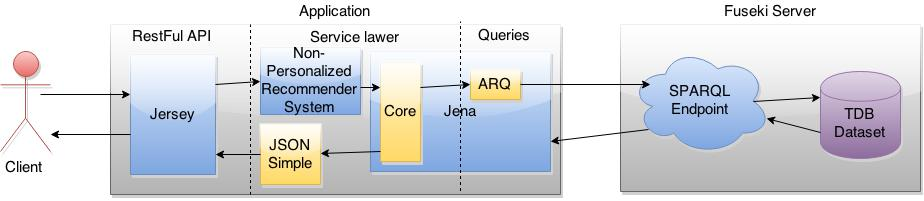
\includegraphics[width=0.8\textwidth,natwidth=610,natheight=642]{explotacion}
    \caption{Arquitectura de la aplicación}
    \label{figure:explotacion}
\end{figure}

\begin{enumerate}
 \item API Restful: Que provee una API mediante la utilización del framework Jersey. Esto evitó 
 que se requiera utilizar una interfaz gráfica que no cumple ningún aporte a los objetivos de esta tesis.
 \item Service: Que proporciona la funcionalidad de la aplicación, generando la estructura de los 
 rankings en el sistema de recomendación, para luego utilizar el framework Jena que modela y proveé la información 
 solicitada por el sistema. 
 
 También posee una librería que mapea la información otorgada pro Jena a Strings JSON que pueden ser 
 devueltos por la API.
 \item Queries: Por último se encuentra la capa queries, que se encarga de obtener los datos del dataset 
 mediante consultas SPARQL generadas por la librería ARQ del framework Jena. Dicha capa será la encargada 
 de interactuar con el SPARQL Endpoint disponible por el servidor Fuseki.
\end{enumerate}